\documentclass[a4paper, 11 pt, conference]{IEEEtran}  % Comment this line out if you need a4paper

\usepackage[utf8]{inputenc}
\usepackage{times} % assumes new font selection scheme installed
\usepackage{amsmath} % assumes amsmath package installed
\usepackage{amssymb}  % assumes amsmath package installed
\usepackage{bm}
\usepackage{xspace}
\usepackage[draft,inline,nomargin]{fixme}
\usepackage{graphicx}
\usepackage{color}

% \hyphenation{non-zero}

\newcommand{\tn}[1]{\textnormal{#1}}        % Wrapper for \textnormal
\newcommand{\Bern}[2]{\ensuremath{\mathcal{B}^{#1}_{#2}}\xspace}
\newcommand{\Cr}{\ensuremath{\text{Cr}}\xspace}

\title{\LARGE \bf Instrumentation of the da Vinci Robotic Surgical System}


\author{Karl Damkjær Hansen \and Simon Jensen \and Christoffer Sloth \and Rafael Wisniewski% <-this % stops a space
%\thanks{*This work was not supported by any organization}% <-this % stops a space
%\thanks{C. Sloth and R. Wisniewski are with Section of Automation \& Control, Aalborg University, 9220 Aalborg East, Denmark
%        {\tt\small ces@es.aau.dk}, {\tt\small raf@es.aau.dk}.}%
}


\begin{document}



\maketitle
\thispagestyle{empty}
\pagestyle{empty}
\begin{abstract}
This paper details the AAU surgical robot, its hardware and software setup.
\end{abstract}

%%%%%%%%%%%%%%%%%%%%%%%%%%%%%%%%%%%%%%%%%%%%%%%%%%%%%%%%%%%%%%%%%%%%%%%%%%%%%%%%
\section{Introduction}
%\subsection{Why is the topic of interest?}
The development of surgical robots for minimally invasive laparoscopic surgery began in the 1980s, primarily supported by the U.S. Army in e.g. DARPA's Trauma Pod program \cite{ravenSpectrum}. Today's leading manufacturer of surgical robotic systems is Intuitive Surgical Inc. that is an offspring of these projects. Their robotic system called da Vinci Surgical System went into use, after being approved by the FDA around year 2000, and has since then been an important tool in minimally invasive surgery requiring high accuracy.

%"The da Vinci Surgical System is a robotic surgical system made by the American company Intuitive Surgical. Approved by the Food and Drug Administration (FDA) in 2000, it is designed to facilitate complex surgery using a minimally invasive approach, and is controlled by a surgeon from a console. The system is commonly used for prostatectomies, and increasingly for cardiac valve repair and gynecologic surgical procedures.[1][2] "

%"Since FDA approval of the da Vinci over 2200 systems are in place, and over 360 000 procedures were performed on humans worldwide in 2011."

Since the launch of the revolutionary da Vinci Surgical System, the innovation in surgical robots has been very slow, among others, due to patenting by Intuitive Surgical Inc. These patents expire by 2016, opening for competitors to enter the market \cite{intuitivePatents}.
%\subsection{What is the background on previous solutions?}
The vast future potential in surgical robotics has spawned new robots to emerge. Among these robots is the university developed Raven open source surgical robot \cite{ravenDesc}, and the DLR MiroSurge by the German research laboratory DLR.

%\subsection{What is the background on potential solutions?}

%\subsection{What was attempted in the present effort?}

The AAU surgical robot is based on a da Vinci robot that is retrofitted with hardware and software for developing an open source surgical robot similar to the Raven. The purpose of developing this system is to demonstrate the potential for autonomy in surgical robots. Currently, surgical robots possess no autonomy - the surgeon does all decision making and manually controls the robot with joysticks. We envision a semi-autonomous surgical robot, where responsibilities are shared among the surgeon and a computer system, similar to an autopilot in an airplane. To allow the da Vinci robot to be controlled by a computer, a hardware and software system has been developed. This will be explained in this paper.

The paper starts by giving an overview of the physical setup of the da Vinci robot, then the developed hardware system in outlined in Section~\ref{sec:hardware}, and finally the software is detailed in Section~\ref{sec:software}.

\section{Robot}
The AAU surgical robot is a first generation da Vinci Surgical System, modified to allow measurement of all motor currents, velocities, and positions as well as grabbing the video from the stereo endoscope. The designed hardware allows the control of all motors of the robot's four arms, each having 7 degrees of freedom. Figure~\ref{fig:robot} shows a picture of the robot, where it is seen that there are three arms for equipping surgical instruments and one arm for the endoscope.

\begin{figure}
    \centering
       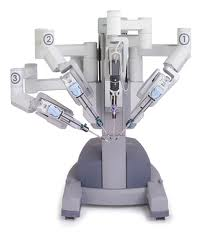
\includegraphics[width=0.5\linewidth]{robot.png}
    \caption{The da Vinci surgical robot. \label{fig:robot}}
\end{figure}

The arms of the robot are configured as shown in Figure~\ref{fig:p4-conceptual}, where the gray section of the robot is fixed during surgery, and the black section can be actuated (three degrees of freedom). The reason for fixing parts of the robot is to fix the robot with respect to the entry holes into the patients body.

\begin{figure}
    \centering
       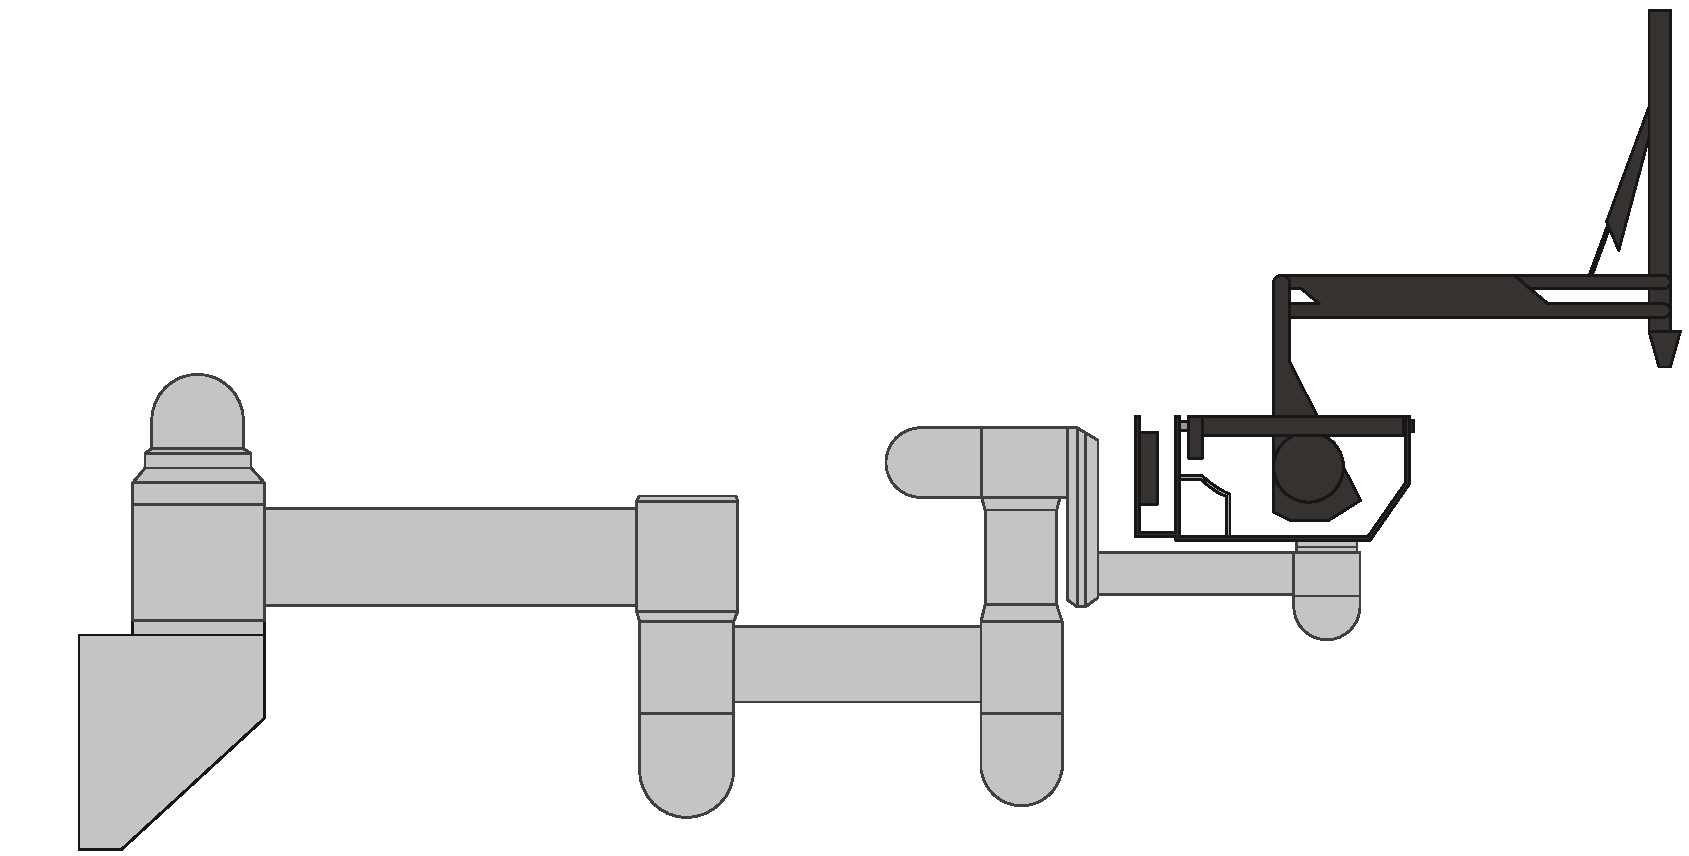
\includegraphics[width=\linewidth]{p4-conceptual.pdf}
    \caption{Sketch of robot arm. \label{fig:p4-conceptual}}
\end{figure}

The final part of the robot is the instrument that comes in several configurations. A gripper instrument is shown in Figure~\ref{fig:gripper} and possesses the last four degrees of freedom.

\begin{figure}
    \centering
       
\includegraphics[width=0.8\linewidth]{endeffector.pdf}
    \caption{Sketch of a gripper instrument. \label{fig:gripper}}
\end{figure}

\section{Hardware}\label{sec:hardware}
Each arm of the robot has 12 degrees of freedom, when including the fixed joints of the arm which are released during configuration.
An embedded computer system is build to control each of these arms and measure their states.
The computer systems consists of two embedded computers which has the two main tasks:
\begin{itemize}
\item Getting measurements (positions, velocities, motor currents) from the sensors on the arm and sending them to a client PC, and
\item getting control reference signals from the PC to drive the motors that controls the motors.
\end{itemize}
Beside these two tasks, the embedded computers enforces security constraints like limiting control values to protect the motors and stopping the motors when the joints reach their limits.

\begin{figure}
\def\svgwidth{0.85\columnwidth}
\input{hardwareRobot.pdf_tex}
\caption{System diagram of the robotic system connected to a client PC.}
\end{figure}

A surgical robot is a safety critical system.
Therefore, one of the embedded computers is in charge of handling the signals from sensors and actuators, while the other acts as the supervisor; handling error situations and dis-/enabling the motor drivers.

The client PC and the robot are connected via a TCP/IP network.
This may present timing problems, as the network may loose packages that must be retransmitted or the network may simply present a delay.
However, this interface is very convenient, as it is ever present on most computers.
The timing problems can be reduced by directly connecting the client and the robot with out any other computers on the network.
But in contrast, the system will natively support remote surgery, where the client PC may be located far away from the robot.


\section{Software}\label{sec:software}
All the higher level functions are handled in the client computer.
These functions are characterized as processes which are not possible to run in real-time, require significant computing power, and/or have loose timing constraints.
These functions are path planning, user interaction, and position control loops.
Low level functions are handled in the da Vinci embedded computers.
These processes all run in real-time and include the speed and current control loops and system error checking.

The interface between the embedded computers and the client is based on TCP/IP connections with a JSON based serialization protocol.

The JSON based protocol is a compromise between a packet size optimization and a protocol that is easy to implement and debug.
The JSON serialization \cite{ecma404} provides a human readable format which is self descriptive but rather compact compared to e.g. XML.
% The JSON format is designed to provide highly self-descriptive messages for REST applications on the Internet, but this typically requires several well-named fields in a hiearcial structure.
% In this application it is not necessary to interpret each message individually, so a descriptive initialization message is sent when the client connects to the robot, and after that the subsequent messages simply holds values in the order defined in the initial message.

As shown in Figure~\ref{fig:control_structure}, there is a cascaded control structure for each of the joints of the robot. Depending on the needs of the researcher, the controllers can either run entirely on the client PC, or the velocity and current controller can be run in the embedded computers.

The software on the client PC is build on the ROS robotic middleware, which provides visualization of the robot, inverse kinematics computations, image processing, and path planning.
Further, a physics simulation of the robot is being developed to run in the Gazebo robot simulator.

\begin{figure}
  \input{controlRobot.pdf_tex}
  \caption{The cascaded control structure of a single joint.}
  \label{fig:control_structure}
\end{figure}

\bibliographystyle{IEEEtran}
\bibliography{bibliography}



\end{document}
